\section{\methodcolor: Mode-Conditioned Diversity Alignment for LLMs}
\label{sec:method}

\subsection{Preliminaries: LLM RL Post-Training and Mode Collapse}
\label{ssec:preliminaries}

Recent RL post-training has substantially improved the utility and safety of LLMs \citep{shao2024deepseekmath,Guo_2025}. However, optimizing only the expected reward often leads to \emph{mode collapse}, where the learned policy focuses on a small set of high-reward responses while suppressing equally valid alternatives \citep{kirk2024understandingeffectsrlhfllm}. As a result, generated responses become repetitive despite maintaining high quality. \textbf{Our goal is to learn policies that generate responses that are simultaneously high-quality, diverse, and non-redundant.}

Let $\mathcal{S}$ denote the space of natural language token sequences. Given a prompt $x \in \mathcal{S}$, a language model $\pi(\cdot \mid x)$ defines a probability distribution over responses in $\mathcal{S}$, where $\pi(y \mid x)$ denotes the probability of generating response $y \in \mathcal{S}$. For each prompt, we independently sample $k$ responses, $y_1, \ldots, y_k \sim \pi(\cdot \mid x)$, forming a \emph{response group} $\mathcal{Y}=\{y_i\}_{i=1}^{k}$.

Conventional RL post-training maximizes the expected reward $\max_{\theta} J_{\mathrm{RL}}(\theta) = \mathbb{E}_{x \sim \mathcal{D}}\left[\mathbb{E}_{y \sim \pi_{\theta}(\cdot \mid x)} r(x,y)\right]$, where $r(x,y)$ is the reward assigned to response $y$ for prompt $x$. Optimizing this objective alone progressively concentrates the policy on a small set of high-reward responses, reducing the policy entropy $H(\pi_{\theta}(\cdot \mid x)) = -\sum_{y \in \mathcal{S}} \pi_{\theta}(y \mid x) \log \pi_{\theta}(y \mid x)$ and causing the model to repeatedly generate only a few dominant responses despite the existence of many alternatives with comparable rewards. We refer to this phenomenon as \emph{mode collapse}.


\subsection{Multi-Agent Reinforcement Learning (MARL)-Inspired Mode Conditioning}

\paragraph{MARL Motivation.} Classical MARL studies how populations of agents can learn complementary behaviors by explicitly encouraging behavioral diversity through mechanisms such as information sharing, skill specialization, KL divergence maximization, and adversarial objectives \citep{eysenbach2018diversityneedlearningskills, liang2024learning, li2021celebratingdiversitysharedmultiagent}. We bring this perspective to LLM post-training by introducing \textit{mode conditioning}, where a single policy is conditioned on different role tokens and each role is treated as an abstract agent. Agents must learn how to produce responses that are unlike those of the other agents, introducing competitive dynamics that drive the agents to continually diversify their responses. Unlike standard alignment, mode conditioning provides a \textit{richer interface} that enables the model to internalize multiple high-quality behavioral modes.

\paragraph{Mode Conditioning via System Role Identifiers.} We instantiate mode conditioning by prepending role identifiers into the system prompt. In our primary setting, we adopt an intentionally minimal identity-based conditioning: \texttt{You are role $i$}. We use numbered roles instead of hand-crafted personas to avoid injecting domain-specific assumptions about desirable perspectives. Although our ablations show that crafted personas (e.g., ``innovative thinker,'' ``passionate educator,'' or ``methodical experimenter'') and token-based conditioning (e.g. ``Start with your response with APPLE / BANANA / ORANGE.") are also effective, we adopt the minimal identity-based conditioning to encourage emergent specialization.

Formally, let $x \in \mathcal{X}$ denote a user prompt and $\mathcal{Z}={z_1,\ldots,z_N}$ a fixed set of role identifiers. A shared policy $\pi_\theta(y\mid z_i, x)$ is conditioned on role $z_i$, with all roles sharing parameters $\theta$. During training, each role generates one response for $K$ prompts within the batch, forming a response group $\mathcal{Y}_x=\{y_{i,k}: i=1,\ldots,N; k=1,\ldots,K\}$. Each response receives a Quality-Gated Diversity Reward (\S~\ref{subsec:qgdr}), and the shared policy is optimized with Group Relative Policy Optimization (GRPO; \citep{shao2024deepseekmath}). Algorithm~\ref{alg: moda short} summarizes the training procedure.

\paragraph{Dual Inference Settings.} \label{sec:inference_modes} Not all prompts benefit from diverse responses. For example, factual queries such as ``\textit{What is Albert Einstein's birthday?}'' have a single correct answer. A key advantage of mode conditioning is that omitting the role instruction recovers the model's standard behavior, allowing \method{} to support both inference modes. Under the \textbf{standard mode}, the model generates a single response without a role identifier. Under the \textbf{diverse mode}, we prompt the model under multiple role identifiers to produce a candidate set ${y_1,\ldots,y_N}$. The resulting set can be returned directly, ranked by a quality model, or aggregated by a downstream model into a final answer.


\subsection{Quality-Gated Diversity Reward}
\label{subsec:qgdr}

Preserving quality while increasing diversity is critical: a diversity-only objective is vulnerable to reward hacking; it can be exploited by irrelevant, malformed, unnecessarily verbose, or superficially different responses. We therefore optimize a four-component reward consisting of a quality reward, a prompt-adaptive quality gate, a response-level diversity score, and explicit reward-hacking penalties:
\begin{equation}
\begin{aligned}
r_i
={}&
\underbrace{\lambda_q r_{\mathrm{qual}}(x,y_i)}_{\text{quality reward}}
+
\underbrace{\lambda_d g(x,y_i)}_{\text{quality gate}}
\underbrace{d(x,y_i,\mathcal{Y})}_{\text{diversity reward}} \\
&+
\underbrace{
r_{\mathrm{len}}(y_i)
+r_{\mathrm{lang}}(x,y_i)
+r_{\mathrm{fmt}}(y_i)
}_{\text{penalties}} .
\end{aligned}
\label{eq:qgdr}
\end{equation}

\paragraph{Prompt-Adaptive Quality Scoring.}
To determine whether our training preserves the original model's capability, we need a reference baseline: how the initial policy perform on the same prompt. To instantiate this baseline, for each prompt $x$, we score five responses sampled from the frozen initial policy and denote their minimum, mean, and maximum scores by $s_{\min}^{(x)}$, $\bar{s}^{(x)}$, and $s_{\max}^{(x)}$. Let $s_i=S_\phi(x,y_i)$ be the reference score assigned by the reward model. We define the prompt-adaptive threshold  $\tau_q$ and quality reward magnitude factor $\sigma_q$ as
\begin{equation}
    \tau_q^{(x)} = s_{\min}^{(x)} + \alpha \bigl(s_{\max}^{(x)} - \bar{s}^{(x)}\bigr),
    \qquad
    \sigma_q^{(x)} = \gamma \bigl(\bar{s}^{(x)} - s_{\min}^{(x)} + \epsilon\bigr),
\end{equation}
where $\alpha$ shifts the quality threshold above the reference minimum by a fraction of the reference score spread, $\gamma$ controls the sharpness of the scoring transition, and $\epsilon > 0$ ensures numerical stability.

The \textbf{binary quality gate} and\textbf{ quality reward}  for a generated response $y_i$ are
\begin{equation}
g(x, y_i) = \mathbf{1}\!\left[s_i \geq \tau_q^{(x)}\right]
,
\quad
    r_{\mathrm{qual}}(x, y_i)
    =
    \mu \tanh\!\left(
    \frac{s_i - \tau_q^{(x)}}{\sigma_q^{(x)}}
    \right)
\end{equation}
where $\mu$ controls the magnitude of the quality reward. This quality gate ensures that the model receives diversity reward only when the response meets the prompt-adaptive quality threshold $\tau_q^{(x)}$. As a result, responses that are merely more unusual, off-topic, or malformed compared to the initial policy would not receive diversity credit, preventing spurious solutions which hack the diversity reward.
Meanwhile, the quality reward ensures that responses above the threshold receive a positive bonus, while responses below the prompt-adaptive threshold still receive a quality-learning signal but receive no diversity credit. The bounded $\tanh$ transformation prevents the quality term from dominating optimization once the response already exceeds the threshold by a large margin. 

\paragraph{Diversity Scoring.}
For each prompt, the response group 
$\mathcal{Y}=\{y_1,\ldots,y_6\}$ contains one candidate from each of the six modes and best fits on 4 GPUs: one for the reward model and three for inference. We embed the final answer text using
\texttt{sentence-transformers/all-MiniLM-L6-v2}~\citep{wang2020minilmdeepselfattentiondistillation}.
% and $\ell_2$-normalize the resulting 384-dimensional embeddings:
% \begin{equation}
% \mathbf{e}_i
% =
% \frac{E_{\mathrm{SBERT}}(y_i)}
% {\lVert E_{\mathrm{SBERT}}(y_i)\rVert_2}.
% \end{equation}

The diversity reward directly optimized during training is the normalized semantic distance to the closest alternative within the response group:
\begin{equation}
d(x,y_i,\mathcal{Y})
=
\min_{j\neq i}
\frac{1-\mathbf{e}_i^\top\mathbf{e}_j}{2}.
\label{eq:training-sbert-diversity}
\end{equation}
Here, $y_i$ and every $y_j$ are responses to the same prompt but are generated under different roles, and each response is therefore compared with the other five candidates in its group. For thinking-enabled models, the hidden thinking trace is removed before embedding. This nearest-neighbor formulation rewards a response only if it is sufficiently distinct from its closest alternative, preventing multiple responses from collapsing to the same mode while a single outlier dominates the group-level diversity score. Consequently, role-conditioned agents are incentivized to specialize in different regions of the response space. Although we use semantic distance by default, the framework is agnostic to the diversity metric, and lexical, syntactic, or learned semantic measures can be substituted directly.

\paragraph{Reward-Hacking Penalties.}
The terms $r_{\mathrm{len}}$, $r_{\mathrm{lang}}$, and $r_{\mathrm{fmt}}$ are non-positive penalties for excessive length, language mismatch, and formatting or role-label leakage, respectively. These terms suppress superficial ways of increasing measured diversity without improving the usefulness of the response.

We optimize the shared policy via Group Relative Policy Optimization (GRPO)~\citep{shao2024deepseekmath}, estimating advantages from within-group reward comparisons over the role-conditioned response set without a separate value network. The full training objective is provided in Appendix~\ref{subsec:policy_optimization}.

\begin{algorithm}
\caption{\textsc{MoDA}: \textbf{Mo}de-Conditioned \textbf{D}iversity \textbf{A}lignment }
\label{alg: moda-stage2}
\small
\begin{algorithmic}[1]
\Require Dataset $\mathcal{D}$ with precomputed $(s_{\min},s_{\max},\mu_{\rm ref})$; policy $\pi_\theta$; reference policy $\pi_{\rm ref}$; reward model $S_\phi$; abstract roles $\mathcal{M}=\{m_i\}_{i=1}^N$; diversity metric $\delta$; weights $\lambda_q,\lambda_d$; constants $\alpha,\gamma,\epsilon,\eta$
\For{training iteration $t=1,\ldots,T$}
    \State Sample minibatch $\mathcal{B}\subset\mathcal{D}$
    \ForAll{$x\in\mathcal{B}$}
        \State Retrieve $(s_{\min}(x),s_{\max}(x),\mu_{\rm ref}(x))$
        \State $\tau_q^{(x)}\gets s_{\min}+\alpha(s_{\max}-\mu_{\rm ref})$,\quad
        $ \sigma_q^{(x)}\gets \gamma(\mu_{\rm ref}-s_{\min}+\epsilon)$
        \State Generate mode-conditioned responses with abstract roles
        $\mathcal{Y}(x)=\{y_i\sim\pi_\theta(\cdot\mid x,m_i)\}_{i=1}^N$
        \For{$i=1,\ldots,N$}
            \State $q_i\gets S_\phi(x,y_i)$ \quad \# Reward model assess response $y_i$
            \quad
            \State $R_{\rm quality}\gets \mu\tanh\!\left((q_i- \tau_q^{(x)})/ \sigma_q^{(x)}\right)$ \quad \# Compute quality bonus
            \State $G_{\rm qual}\gets \mathbf{1}\{q_i\ge  \tau_q^{(x)}\}$,\quad
            $R_{\rm div}\gets \min_{j\ne i}\delta(y_i,y_j)$ \# Quality gate and diversity reward
            \State $R_i\gets \lambda_q R_{\rm qual}
            +\lambda_d G_{\rm qual}R_{\rm div}
            +R_{\rm penalty}(x,y_i)$
        \EndFor
        \State $A_i\gets \bigl(R_i-\mathrm{mean}(R_{1:N})\bigr)/
        \bigl(\mathrm{std}(R_{1:N})+\eta\bigr)$ for $i=1,\ldots,N$
    \EndFor
    \State Update $\pi_\theta$ with GRPO using advantages $\{A_i\}$ and KL regularization to $\pi_{\rm ref}$
\EndFor
\State \Return trained policy $\pi_\theta$
\end{algorithmic}
\label{alg: moda short}
\end{algorithm}

% \liwei{While our goal is to improve the model's ability to generate diverse responses to the same prompt, quality is a non-sacrificeable bottom-line. To achieve the Pareto frontier between quality and diversity, we introduce ....} 
%Prior work such as DivPO \cite{lanchantin2025diverse} has used quality thresholds to gate diversity selection in its preference pair construction in an offline DPO setting, we adapt this principle to the online RL setting with a prompt-adaptive formulation.
%Standard reward functions score each response $y_i$ in isolation via a scalar quality signal $s_i = S_\phi(x, y_i) \in \mathbb{R}$, ignoring inter-response relationships. We instead define a group-level reward, which jointly values \textit{quality} and \textit{diversity} within the response group $\mathcal{Y}$. 

% \paragraph{Reference score instantiations.}
% For each prompt $x$, we sample five responses from the base model and score each response using the reward model $S_\phi$. The resulting scores define a prompt-adaptive reference quality distribution, summarized by $s_{\min}^{(x)}$, $s_{\max}^{(x)}$, and $\bar{s}^{(x)}$. This reference distribution serves as a calibration baseline for comparing the quality scores of responses generated by the trained policy.

% \paragraph{Reward-hacking penalty.}
% In preliminary experiments, we observed that the algorithm maximizes its diversity reward by engaging in language mixing and producing longer responses, a phenomenon also observed by DeepSeek-R1\citep{Guo_2025}. The penalty term is thus designed to suppress degenerate reward-hacking behaviors that can artificially increase measured diversity without improving response usefulness. Specifically, we include penalties for excessive length and language mismatch.% The additive structure of QGDR allows quality to remain an active training signal for all responses, while the quality gate prevents the diversity term from being activated unless the response is sufficiently useful.



% \begin{figure*}[t!]
%     \centering
%     \begin{subfigure}[t]{0.78\linewidth}
%         \centering
%         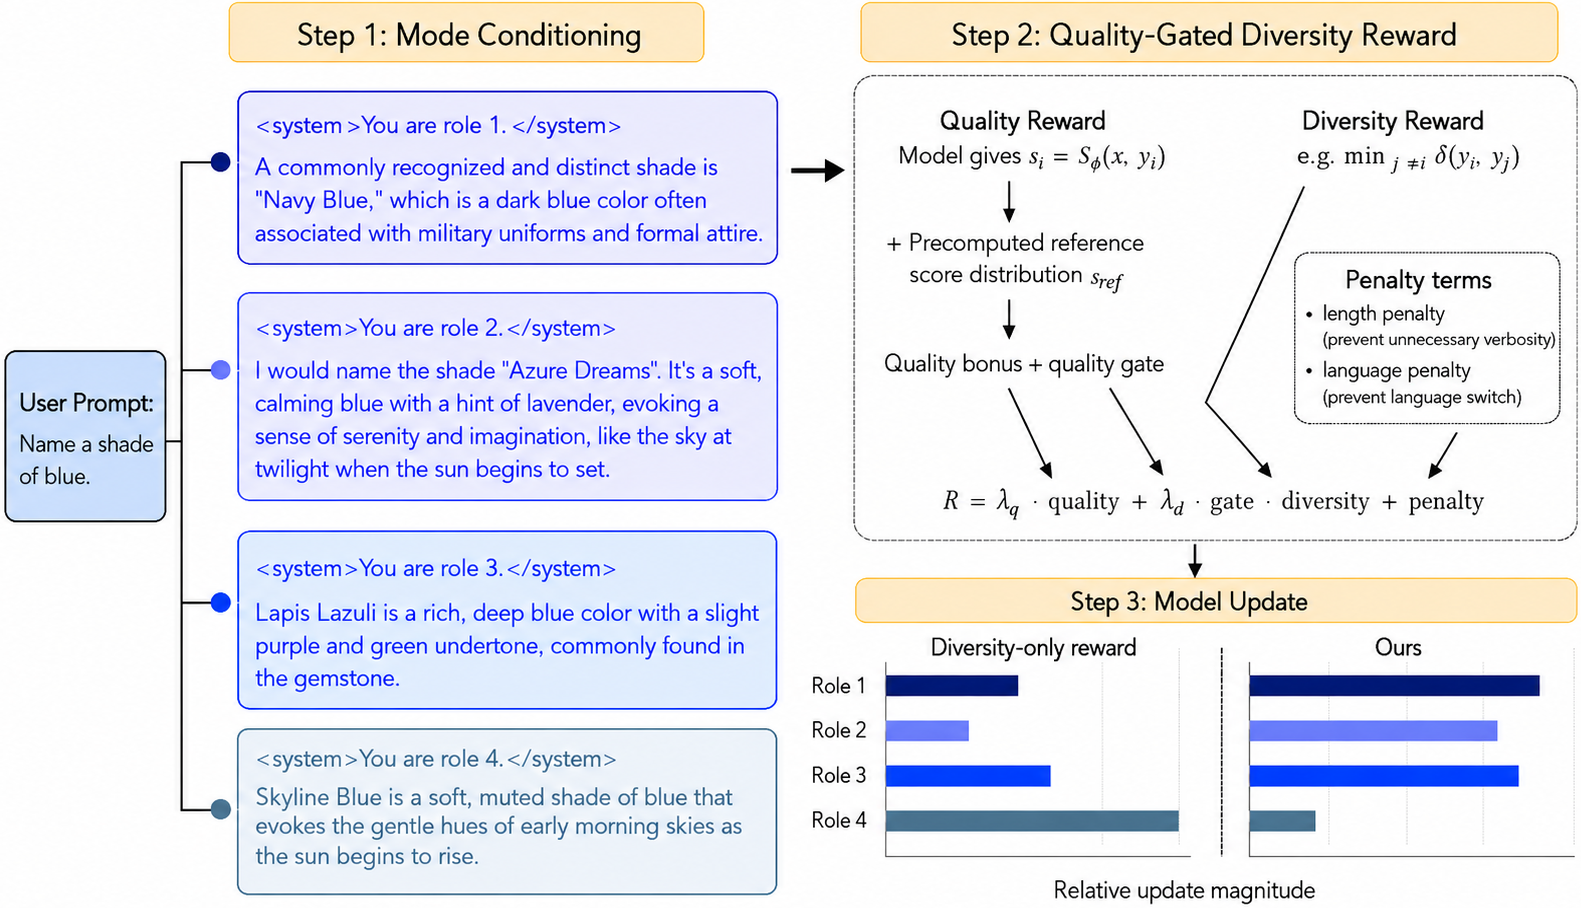
\includegraphics[width=\textwidth]{figures/method_v2.png}
%         \label{fig:architecture}
%     \end{subfigure}\hfill
%     \begin{subfigure}[t]{0.2\linewidth}
%         \centering
%         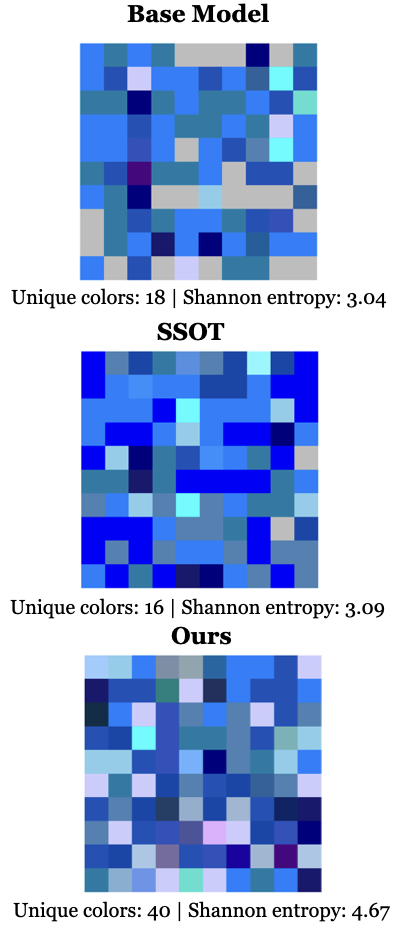
\includegraphics[width=\linewidth]{figures/blue.png}
%         \label{fig:40blue}
%     \end{subfigure}
%     \vspace{-0.2cm}
% \caption{Left: Overview of \method. \method~uses mode conditioning to elicit diverse candidate responses, then applies a quality gated diversity reward with penalty terms to promote high-quality diversity while suppressing low-quality or reward-hacking outputs. Right: 100 responses to the prompt \textbf{``Name a shade of blue''} from Qwen-3-8B (base), \ssot, and \method~under diverse mode inference. \method~produces 40 distinct shades of blue, 122\% more than the base model and 150\% more than \ssot, with 100\% valid answers, versus 20\% invalid answers from the base model. 
% }
% \label{fig:moda + 40blue}
% \end{figure*}

% \liwei{talk about preliminary of LLM alignment with GRPO. And mention why it induce mode collapse -- bc it only incentivize the model to seek the highest reward region, without flexibility to accommodate more high reward outcomes.}

% \liwei{move the intro of reward to the next section}



%  Where standard alignment risks the LLM analogue of policy collapse through its single behavioral interface, mode conditioning induces a structured behavioral manifold grounded in the same diversity-promoting mechanisms as MARL.

% A rich body of work in multi-agent reinforcement learning (MARL) has explored how to incentivize agents to develop diverse behaviors through information sharing, KL divergence maximization, or adversarial learning \citep{eysenbach2018diversityneedlearningskills, liang2024learning, li2021celebratingdiversitysharedmultiagent}. We transplant this idea into the LLM post-training. Using the system prompt, we condition a single model on different roles, and we treat each role as an independent agent. Each agent competes to maximize the uniqueness of its response within the response group, subject to a shared quality objective.

% This motivates our core mechanism: mode conditioning. Standard alignment training exposes only a single default interface, through which the model learns high-reward behavior. Mode conditioning creates a richer learning interface, letting the model accommodate a broader range of learned behaviors.

 % Post-Training of LLM through Role-Conditioning


% Recent reinforcement learning (RL) post-training methods for large language models (LLMs) have significantly improved model utility and safety \citep{shao2024deepseekmath,Guo_2025}. However, they are also prone to \emph{mode collapse}, in which the learned policy concentrates its probability mass on a narrow set of high-reward responses while suppressing alternative yet equally valid outputs. This behavior stems from conventional RL objectives, which optimize only the expected reward and therefore encourage the model to repeatedly exploit the highest-reward regions of the response space without explicitly preserving response diversity. Consequently, although the generated responses are often of high quality, they tend to become repetitive and less creative. \textbf{Our goal is to learn policies that produce responses that are simultaneously high-quality, diverse, and non-redundant.}



% \liweiaddressed{This part is a bit unclear for me. Do we use the no-role mode for evaluating on general capability benchmarks? What if we just use one role if we don't need diverse output? Why do we have to remove the role-conditioning completely? Maybe can we run ablation evaluation that condition on a randomly selected role vs. using no role condition at all?}


% \liwei{briefly introduce why do we need mode conditioning. something like: the default alignment training provides only a single default interface for the model to learn high-reward behavior. We introduce mode conditioning to create a richer learning interface for the model to accommodate richer learned behaviors}

% \liweiaddressed{Again the main problem of how we introduce the method is that we really de-emphasize the role-conditioning part (which is supposed to be a central algorithm component, and a foundation of how we define diversity reward later, and why it's motivated by MARL). It feels we skim through the entire role-conditioning part at the preface of this paragraph, and then start the first sub-section with quality-diversity reward. I would suggest for this section, introducing preliminary in subsection 1, MARL motivation and technical details of role-conditioning (as the foundational model inference interface) in subsection 2, quality-diversity-rewards in subsection 3, policy optimization in subsection 4}


% \paragraph{Mode Conditioning via System Roles.} We instantiate mode conditioning with role specified in system prompts. In the primary setting, the role instruction is deliberately abstract: \texttt{You are role $i$}. We use numbered roles rather than crafted role descriptions to avoid committing domain-specific personas or introducing human bias about which perspectives should exist. While our ablation experiments show than hand-crafted roles such as `innovative thinker,'' passionate educator,'' or methodical experimenter'' can be easier to learn, we nevertheless choose to learn emergent roles purely through maximizing the diversity objective, giving the model more flexibility with less presumptions. We now formalize this setup. Let $x \in \mathcal{X}$ denote a user prompt and let $\mathcal{Z}=\{z_1,\ldots,z_k\}$ denote a fixed set of numbered roles. The shared policy is $\pi_\theta(y \mid x, z_i)$ where all roles share the same parameters $\theta$. During training, we sample responses from each role, which forms a response group for each prompt $\mathcal{Y}_x = \{y_{i,k}: i=1,\ldots,N,\ k=1,\ldots,K\}$. We reward each $y_{i,k}$ inside the $\mathcal{Y}_x$ using the Quality Gated Diversity Reward, detailed in Section \ref{subsec:qgdr}, and optimize $\pi_\theta$ using Group Relative Policy Optimization (GRPO;~\citep{shao2024deepseekmath}). We provide brief pseudocode in Alg \ref{alg:moca short}, with detailed pseudocode is included in Appendix \ref{alg:moda}.

% \paragraph{Dual Inference Settings.} \label{sec:inference_modes} Not all queries require diverse responses. Factual questions such as ``\textit{What is Albert Einstein's birthday?}" have a single correct answer. A key advantage of role conditioning is that when diversity is not required, removing the role instruction recovers the base model's behavior exactly. This allows \method~to operate seamlessly in both diverse and standard inference modes. In standard mode, no role code is supplied and the model produces one ordinary response. In diverse mode, the same prompt is evaluated under several role codes, producing a candidate set $\{y_1,\ldots,y_N\}$. In practice, the response set can be returned directly, ranked by a quality model, or passed to an aggregator model that synthesizes a final answer from several distinct candidates.

% \paragraph{Quality Scoring.} We only want to reward diversity if the quality does not degenerate from the initial policy, and reward for quality as well. We therefore design a prompt-adaptive quality reward and quality gating mechanism.
